 %Game Engines, Game Design, Game Algorithms, Motion Planners, Computational Physics (fluids), Parallel/Grid/Cloud Computing, Human Computer Interaction  

\documentclass[tikz,border=2mm]{standalone}

\begin{document}
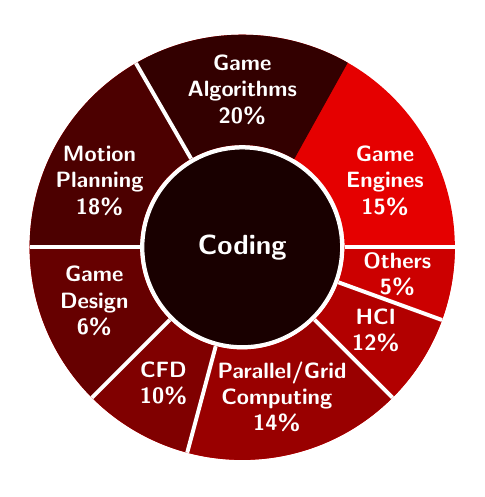
\begin{tikzpicture}[font=\sffamily\bfseries\large, 
     text=white, 
     border/.style={line width=14mm}]
\foreach \angle/\col [remember=\angle as \last (initially 0)] in 
    {360/red!90!black, 340/red!80!black, 315/red!70!black, 255/red!60!black, 225/red!50!black, 180/red!40!black, 120/red!30!black, 60/red!20!black}{    
        \draw[\col, border] (\last:2cm) 
             arc[start angle=\last, end angle=\angle, radius=2cm];
        \draw[white, line width=0.5mm] (\last:1.3)--++(\last:1.4);
}
\node[text width=2.2cm, align=center, font=\sffamily\bfseries\normalsize, draw, circle, minimum width=2.5cm, white, fill=red!10!black] {Coding};
\node[text width=1.1cm, align=center, font=\sffamily\bfseries\footnotesize] at (25:2cm) 
    {Game Engines 15\%};
\node[text width=1.4cm, align=center, font=\sffamily\bfseries\footnotesize] at (90:2cm) 
    {Game Algorithms 20\%};
\node[text width=1.2cm, align=center, font=\sffamily\bfseries\footnotesize] at (155:2cm) 
    {Motion Planning 18\%};
\node[text width=1.1cm, align=center, font=\sffamily\bfseries\footnotesize] at (200:2cm) 
    {Game Design 6\%};    
\node[text width=1.1cm, align=center, font=\sffamily\bfseries\footnotesize] at (240:2cm) 
    {CFD 10\%};
\node[text width=1.5cm, align=center, font=\sffamily\bfseries\footnotesize] at (283:1.95cm) 
    {Parallel/Grid Computing 14\%};       
\node[text width=1.1cm, align=center, font=\sffamily\bfseries\footnotesize] at (328:2cm) 
    {HCI 12\%};
    \node[text width=1.1cm, align=center, font=\sffamily\bfseries\footnotesize] at (350:2cm) 
    {Others 5\%};    
\end{tikzpicture}
\end{document}
